\chapter{Generation of a DSL Syntax} \label{chap:generation_dsl}
\par
The Syntax of the DSL is the most important part of the project, as it is the place in the toolchain, where the modeller actually does his work: writing a model. Therefore the main requirement for the DSL is that the modeller, must be able to express all the functionalities needed for his models. On the other side, the syntax of the DSL must be as straightforward and intuitive as possible, so that the modeller can concentrate on his scientific activity and must only invest a small amount of time to learn and handle the DSL \autocite{dsl:mernik}.
\par
It is difficult to develop a DSL, with such a balance, in one step. Therefore the approach was to develop an easier DSL in the first place. Afterwards this DSL was used to develop simple existing models. Through that development the created DSL syntax could be validated. With this newly gathered modeling experience, it was possible to evaluate the syntax and the missing features of the DSL and to improve it in the next iteration of the same procedure.
The Similie tutorials were used as a starting point, for the first DSL draft. Similie and its tutorials were chosen over the other analysed frameworks because they had a clear structure and were well explained.
\par
With this approach, two DSL drafts were created. After the second draft, we realised that, it would not be possible to create our own DSL. Thus we tried to find another modelling DSL which already covers some needed features and provides us with a clear and structured syntax, which we finally could extend.
\par
In this section the two created drafts are described, then our chosen candidate DSL, Ocelet, is introduced and finally necessary extensions to Ocelet are specified.

\section{First DSL Draft}
\par
The first draft is a DSL that has the necessary functions to describe the bank-account model from the Similie \autocite{dsl:similie_tutorial_bank} tutorial. The attempt was to create a DSL with Xtext, a framework for DSLs, and to bind the DSL with an ontology.  
\par
For this first draft a practical approach was chosen, although this is not essential for a feasibility study. Nevertheless further insights and ideas were gained for the general DSL generation, by making the first steps for creating a DSL with Xtext. Thereby it could finally determined, that any implementation of runnable code from an own DSL, was completely out of scope for this project. This was due that, lots of DSL creation challenges appeared, which were partially hard to solve but mainly consisted of diligence work. These challenges were not relevant for the further proceeding, and therefore we stopped the concrete implementation at some point.\\
Another goal was to bind the DSL with an ontology, by that it would have been shown that if this works for a simple example, the same principle could also be applied for more complicated cases. 

\subsection{Implementation}
\par
To understand the further thoughts, it is necessary to comprehend the Similie Bank model shown in the diagram \ref{fig:simile_bank_account} below:
\begin{figure}[h]
	\centering
	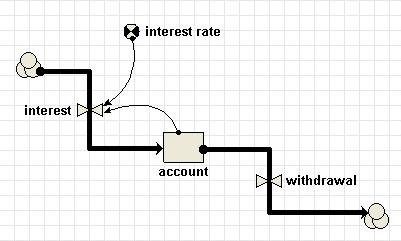
\includegraphics[width=0.7\textwidth]{pics/generation_of_a_dsl/similie_bank_account.png}
	\caption{Simile Bank Account \label{fig:simile_bank_account}}	
\end{figure}
\par
In detail, the diagram shows a compartment with the name $account$, the compartment has a value which represents the account balance. $Account$ has the starting value: $20$. It further shows a variable $interest\:rate$, which has a constant value. In this example it is $0.1$. There are also two flows in the picture. A flow adds or subtracts a certain value of a compartment, depending if it flows into to the compartment or out of it. The value is calculated by a formula the user entered. The two arrows are so called influences, they represent that the value of $account$ and $interest\:rate$ can be used in the formula of the $interest$ flow. The formula of $interest$ is $interest rate * account$ and that of withdrawal is $20$.
\par
Simile can convert this diagram into an executable program, which simulates this bank account. The principle of that program is, that every value will be recalculated for each timestep, based on the previous value. The user can enter how many timesteps will be calculated. In pseudo-code the main logic of the program could look like this:
\begin{verbatim}
interest_rate = 0.1
account = 20
timestep = 100
for each timestep:
	account = account + (interest rate * account)
	account = account - (20)
\end{verbatim}
\par
Of course this is not everything Simile does, as it is also responsible for I/O like drawing diagrams and so on. Nevertheless it should show, what is done at the first glance.\\
Our first DSL had the goal to be able to represent this diagram textually, so the bank account example described with the the DSL looks like the following:
\begin{verbatim}
Model bankAccount:
Container account INT = 200;
FlowIN INT interest TO account = interest_rate * account;
FlowOUT INT withdrawal FROM account = 20;
Conjunction interest_rate -- interest;
Conjunction  account -- interest;
variable INT interest_rate  = 0.1 ;
\end{verbatim}
\par
This way of describing a model has several flaws, which mostly result  from the fact that the DSL tries to mimic functionality that works for a visual modelling but not necessarily for a text based description of a model.
\par
The first problem is the use of conjunctions, which represent influences in Similie. In Similie they are needed to make values visible in the components where they should be used. For example: if the arrow from $account$ to $interest$ does not exist, the value from $account$ could not be used in the formula to calculate $interest$.\\
Therefore in our syntax the conjunctions are used to define the scope of use of variables and containers. This concept is widely known in programming as visibility rules. Defining every conjunction between variables, flows and containers with 1to1 relations is not practicable. If such visibility rules are needed a more effective way must be found.
These relationships serve another purpose in the execution of the model. By calculating the dependencies, the execution order in a model is determined. Without dependency definitions by the modeler, the calculation of dependencies and the execution of the model is bound to much more effort in the code generator.
\par
The next problem is the readability. A direct conversion of a visual modeling language to a textual does not produce a DSL with a readability that is necessary for a useful DSL. The conclusion is that a new concept for a DSL is necessary.
\par
The description of a model with a DSL is followed by the generation of executable code. XText already offers a mechanism to implement such a code generator, but the conceptual problems were too complex, so that no executable code generation was achieved. To overcome these conceptual complexity, deeper experience with code generation and compilers is needed. Nevertheless, with this experiment with XText we got a feeling, on what is possible with a DSL, and what is not. 
\par
An effort to find a way to integrate unit conversion with the help of ontologies into the code generation led to a small example, a Java standalone program, where the information on how to convert degree Kelvin to Celsius and vice versa is extracted from NASA Sweet ontologies. The example could not be tested with the DSL because of the problems with the code generator, but experience with information extraction from ontologies was gained. In principle it is possible to make such connections to the ontologies and to bind the data types with semantic. 
\par
The result of this example is that the code generation is out of scope for this project and that a new DSL definition is necessary, because a textual DSL has other requirements than a visual modeling like Simile. Though we went on to the second DSL draft.

\subsection{Second DSL Draft} \label{sec:second_dsl_draft}
\par
In our second DSL draft we decided to follow the explanations in the Paper ``Declarative Modelling'' from \autocite{dsl:muetzelfeldt}. So we have chosen to define our DSL in a declarative way. That means that, in the most cases, there is no need to write instructions how to calculate some values. The goal is to describe all calculations with describe statements as a mathematical formula. These describe-statements of the calculations can be separated from the concrete model. That means the concrete model uses the formulas which was described earlier or are available in a database/ontologie.
\par
Each describe-statement defines a mapping between a new value set and a value set that is used to generate it. This idea includes some advantages known from functional programming languages:
\begin{enumerate}
	\item Facilitated model verification: In fact that Describe Statements does not accesses the memory, since they are defined declaratively.
	\item Usability: The modeller, often with a strong mathematical background, is able to write his models in a way that is familiar to him by using formulas instead of instructions. The fact that the code is easier to write accompanies the advantages that the code is also easier to read.
\end{enumerate}
Once we have described all necessary mathematical functions/mappings in our DSL we have to bring these mappings together in an executable model. To run a model  we need to describe each iteration. At this point we break with the declarative paradigm and use an imperative style to define each iterations.
%TODO Referenz suchen.
An imperative approach brings the advantage that we have an random access to values calculated in previous iterations and we are able to pass the results of the current iteration to the next iteration. \\
The bank account model implemented in the DSL would look something like this:
%TODO Syntax hervorheben
\begin{verbatim}
describe interest_rate depends on timestep as 1 end
describe q depends on interest_rate as 1+interest_rate/100 end
describe withdrawal depends on timestep as 50 end
describe balance depends on q, withdrawal, old_balance as
old_balance * q - withdrawal
end
run simulation from 1..10
    init tmp_balance = 1000 do
	tmp_balance = balance(q(interest_rate), withdrawal, tmp_balance)
end
\end{verbatim}
\par
In the code above it is recognizable that the $describe$ statement is used to define a mathematical function. In the example $interest\_rate$ depends on timestep. Described in mathematical terms:\\
$interest\_rate(timestep) : \mathbb{N} \rightarrow  \mathbb{R}$
\par
At the moment $interest\_rate$ maps every timestep to the value 1 but in reality the $interest\_rate$ changes in time. There is a possibility to describe the changes with a formula but in many cases there is no structure in the changes. For the case of $interest\_rate$ it should not be only possible to write mathematical expressions after the $describe$ statement, further it should possible to read the desired values from an array, a submodel or a database. So the $describe$ statement provides a way to plug datasources or other models into our models.
\par
Up to that point, we ignored the connection between the ontology and the syntax of the DSL. Nevertheless we wanted to try to build a sample model with that DSL, to get a feeling for it and perhaps get an idea how we could realise the connection to the ontology. So in the next step we tried to write a predator-prey model with the DSL.
\par
The predator-prey model was build after that one used in \autocite{dsl:dynamo}. The model with our syntax can be found in the [appendix].
%TODO ist das im Anhang etc. 
The resulting code is not finished but already bloated and therefore not readable and unintuitive.
\par
Because of those two points, missing connection to an ontologie and intuitiveness, we decided to research an already existing DSL for environmental modelling, which we could use as template.

\subsection{Ocelet}
\par
The result of that search was Ocelet. Ocelet is a modeling language and a development environment for landscape models. It was developed in the scope of the STAMP project, which stands for Modelling dynamic landscapes with Spatial, Temporal And Multi-scale Primitives. \autocite{dsl:ocelet-wiki} The project is supported by the ANR, the Agence Nationale de la Recherche. It started in 2007 and had a duration of 42 months, after which it was abandoned and is not in further development. We could not find out, if a follow-up project exists.
\par
The following information about Ocelet were found in \autocite{dsl:ocelet-design}. The goal of Ocelet is to allow the domain experts to concentrate on the conceptual model. The task of the transformation of the model to an executable implementation is left to an dedicated software tool.  \\
Though the design of Ocelet has the following two main points.
\begin{enumerate}
	\item It provides concepts adapted for the modelling processes, especially in the landscape sector.
	\item It must have underlying operational semantics that are required to automatically generate code and run simulations, which correspond to the models written in the Ocelet programming language. This means that Java code is generated from Ocelet code, thus a code generator are needed.
\end{enumerate}
To make the modeler’s work easier, Ocelet provides a model building environment, which enables syntax analysing and type verification, which is standard in most other common programming languages. \\
Furthermore the model needs to be executed, so Ocelet also provides a program execution platform based on component-service technologies. \\
A schematic overview of Ocelet can be seen in the diagram \ref{fig:ocelet_modelling_and_simulation_framework} below, it is taken from \autocite{dsl:ocelet-design}.
\begin{figure}[h]
	\centering
	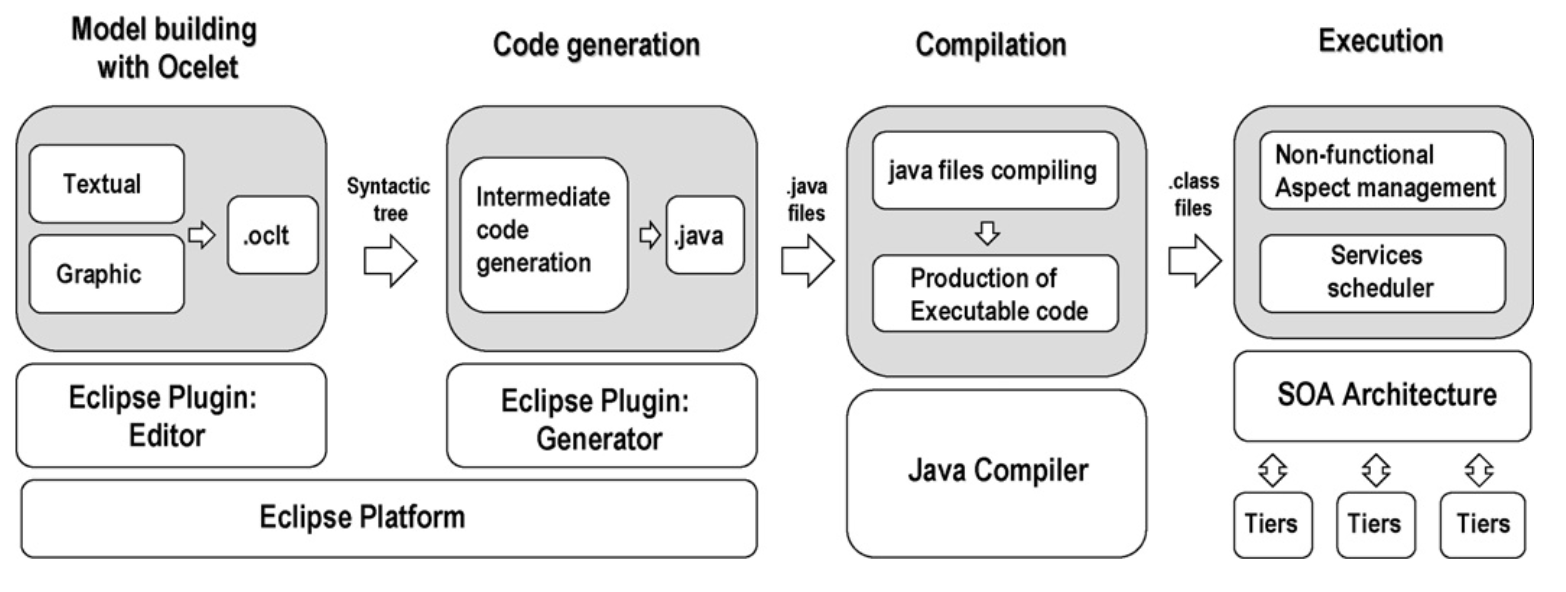
\includegraphics[width=1.0\textwidth]{pics/ocelet/ocelet_modelling_and_simulation_framework.png}
	\caption{A schematic overview of Ocelet \label{fig:ocelet_modelling_and_simulation_framework}}	
\end{figure}

\subsubsection{Modelling paradigm}
\par
As already described Ocelet is an own DSL, where the code is translated to Java, which then can be executed on the computer.\\
Ocelet was build around of 5 main concepts:
\begin{itemize}
	\item entity
	\item service
	\item relation
	\item scenario
	\item datafacer
\end{itemize}
These concepts are further explained in more detail subsequently. Of course Ocelet also knows other common concepts like arguments, properties and numbers, which will not be explained in detail in this document.
\par
The following definitions of the 5 main concepts are taken from \autocite{dsl:ocelet-onto} and \autocite{dsl:ocelet-design} respectively.
\emph{
\paragraph{Entity}
Entities are basic modelling parts that can be put together to build a model. A whole model is, as such, also an entity. An entity can contain other entities, and is then called a composite entity. Entities that do not contain other entities are called atomic entities. An entity is able to store information using attributes. An entity communicates with its environment through input and output ports named services.\\
For example: A forest can be modelled by a composite entity that contains tree entities which are part of the forest. And each tree can have an age attribute.
\paragraph{Service}
A service is a communication port of an entity. It is an input service when it accepts input values or events from other entities and it is an output service when it exports values or events to other entities.\\
Services are defined like functions: they have a name, accept arguments, can produce results.
\paragraph{Relation}
A relation is the expression of how a set of entities relate to each other at a given moment. Hence a relation definition describes which entities can be related and also contains a functional part which describes what is happening when they interact.
\paragraph{Scenario}
A scenario gives a description of which actions and relations within a composite entity have to be activated, and when. The relations in turn put selected entities in interaction in space and time. The scenario therefore expresses the spatial and temporal internal behaviour of a composite entity by managing the entities and relations it contains. For example, a ten-year evolution scenario embedded in a village entity could describe the extension of the village by a few houses every year, taking in account population growth and several policy rules that govern spatial expansion. The ten-year scenario could also be composed of yearly evolution scenarios.
\paragraph{Datafacer}
A datafacer is a component through which entities access data. The aim of datafacers is to abstract access methods to the entities. In the domain of geographical information, a datafacer can take the form of an external database, a satellite image repository or an internal logfile.
}
\par
In \autocite{dsl:ocelet-design} the creators of Ocelet show that these five concepts are enough to represent most of the situations, which occur in dynamic landscape modeling. Although it is not proven if these concepts are also sufficient to represent most environmental models, which are not directly connected to the landscape.

\subsubsection{Ocelet and Ontologies}
\par
According to \autocite{dsl:ocelet-design} an ontology can be mapped to Ocelet code and vice versa. This is shown in diagram \ref{fig:ocelet_and_ontologies}.
\begin{figure}[h]
	\centering
	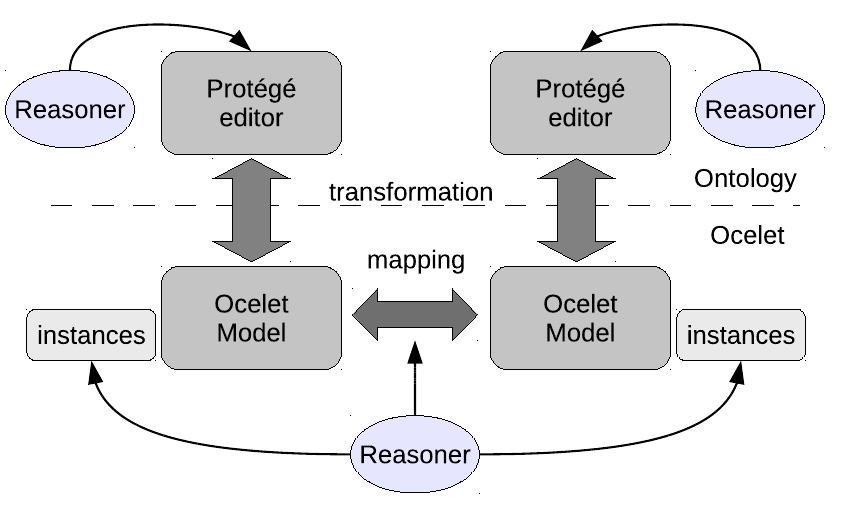
\includegraphics[width=0.7\textwidth]{pics/ocelet/ocelet_and_ontologies.png}
	\caption{Ocelet models and Ontologies  \label{fig:ocelet_and_ontologies}}	
\end{figure}
\par
In the image it is shown that a model can be mapped to an equivalent model in an ontology. Furthermore the mapping is fully automated and therefore does not require any actions of the end-user. This has the advantage that the model can be checked for inconsistencies with a reasoner. Although the modeler can be warned about such inconsistencies, it is not possible, to automate the repair process, as it is a nondeterministic process.  
\par
Another advantage is that parts of one model can be easily reused in other models, as for example an entity in one model can be an equivalent, specialisation or generalization of an entity in an other model.

\subsubsection{Missing features of Ocelet}
\par
For our use, Ocelet has two main shortcomings. In the first place, Ocelet does not follow an universal approach as it only focuses on landscape modelling. Secondly, Ocelet models can be reasoned with ontologies, but this feature is not as extensive as we need it.

\par
In the next section, we describe therefore how Ocelet could be enhanced for our needs.

\section{Needed enhancements of Ocelet}
\par
As already described Ocelet has two main shortcomings, a focus on landscape modelling and a lack of semantic. Besides of these it also has a few minor shortcomings. The created model has no metadata, the use of nested arrays and more complex data structures is not clear and there could be some improvements to handle different timesteps. Possible solutions to these problems will be described in this section, whereas the problem with the semantics will be discussed in the next section.
\subsection{Metadata}
\par
As described in the previous chapter, annotations can be used to add metadata to a model. A list of every possible annotation can not be provided here, but has to be elaborated in a future work. To show how the use of annotations could look like, two possible annotations, @IN and @OUT, are introduced here. They specify if a variable is an input or an output parameter of a component. They can be used to define the interface of a component.
\par
Thus a rabbit entity from a predator-prey model could look like the following:
\begin{lstlisting}
entity rabbits{
    @IN property population
    @IN property reproduction = 0.01   

    Service produce()
}
\end{lstlisting}
The creation of a new rabbit entity could look like this:
\begin{lstlisting}
scenario Main{
    r = rabbit(50);
}
\end{lstlisting}
But the input parameter could also be nested, in such way the input parameter is forwarded over multiple components:
\begin{lstlisting}
scenario Main{
    @IN parameter rabbitPopulation;
    @OUT parameter finalRabbitPopulation;
    r = rabbit(rabbitPopulation);
    .
    .
    .
    return finalRabbitPopulation;
}
\end{lstlisting}
%TODO code rahmen wegmachen
\par
In this case. the scenario awaits the input parameters as user input, as it is similarly done in OMS, and then forwards the parameters to its entities. Additionally, the @OUT annotation specifies the variable which will be returned as result of the model, namely the final rabbit population.

\subsection{Nested arrays}
\par
Ocelet has a shortcoming on more complex data structures, thus it must be enhanced in that direction.\\
This should be solved with data structure paradigms which are known from other programming languages. Among these, arrays and two dimensional arrays are the most basic data structures and should therefore be used. Furthermore if the possibility exists to nest arrays, this can be used as foundation of other more complex data structures, as those often build up upon them. Thus the nesting of arrays is the first step, in direction of more complex data structures. 
\par
In the following example it is shown how satellite pictures and their metadata could be represented with grids, also known as a two dimensional array.\\
In general a satellite picture is not a single big picture, but it is assembled from some single smaller pictures. To form the actual pictures these parts can be arranged in a grid. How this could be done with our syntax is shown below. 
\par
An entity $SatellitePicture$ and $SatellitePicturePart$ is given:
\begin{lstlisting}
entity SatellitePicture{
    property Satellite s;
    property SatellitePicturePart[][] parts;
    ...
}

entity SatellitePicturePart{
    property Coordinates l;
    property Picture p;
    ...
}
\end{lstlisting}
\par
The entity $SatellitePicture$ contains some metadata of the picture and the needed parts to assemble the picture. These parts are already ordered in a grid. The entity $SatellitePicturePart$ contains the actual pictures and also some metadata about the single part. For example the coordinates, which are needed to put the part on the right place in the grid.
\par
The grid could be allocated with: $parts = new SatellitePicturePart[n][m];$
Where $n$ and $m$ are two integers to define the size of the grid.
\par
To give the modeler the possibility to create such data structures, a first implementation of our project, should contain arrays and the possibility to nest them. Though, as it is very tedious to work only with arrays and nested arrays, other data structures which are known from Java (like arraylists) and other programming languages, should be build in the subsequent implementations.
\par
Up to this point the arrays are only allocated but are still empty and do not contain any data. They could be either initialized by the modeller, or filled via Ocelet’s datafacers or via SQL statements. For the later, it has to be proven if it is advantageous to build this functionality into the language, or if it is better to implement the SQL queries with the help of a datafacer.
\subsection{Access past timesteps}
\par
According to our knowledge, the two following features have till now not been described in a environmental modelling context. However, we think that it might be a helpful functionality.
The idea of the first feature is, that it should be possible to access every value of every variable from every past, speak already calculated, timestep. To realise this the variables have to be enhanced in such way, that they are associative arrays, where a certain time step (so to speak the date \footnote{In this section, date has not the common definition, but is something similar to the Java class Date. This means that it specifies the time and day.} of the time step) is the key and the value is the actual value of the variable. To simplify the modeler’s work, this has to be hidden from him, so that he can easily use this additional functionality. Thus if he uses the variable in a normal way, the last saved value will be used. But he can also use the variable with the appendix $.from(Date)$, in this case the variable returns the value of that date. If this feature is considered useful in general, it has to be worked out, as some questions are still open. For example: what happens if no value is available for the stated date. In that case, should it always be an error, or should some interpolation be used.
\par
The second idea is that a more descriptive way of writing a for-loop should be introduced. This loop could have the following structure:\\
$for(from\_date,\, to\_date,\, granularity)$, where $from\_date$ and $to\_date$ are two dates and the granularity is a unit to describe time (second, day, year etc...). The loop would then iterate from the $from\_date$ to the $to\_date$. Thus the first timestep would be the $from\_date$. The second time step would be the first date added up by the granularity. The third time step would be the second date added up by the granularity and so on until the $to\_date$ is reached or passed, at this point the loop will break. To access the date of the current timeStep the variable $currentTimeStep$ can be used. For the loop there are also some important  open questions: how could a nested loop be realised and what arithmetic on the $currentTimeStep$ variable should be possible? For example, if the $currentTimeStep$ is the $24.12.2006$ and the granularity is $hour$, should $currentTimeStep+1$ result in $24.12.2006 01:00 am$?
\par
The two ideas complement each other, as in the first idea one remaining question is, when and how should the data be written into the associative array. With the timestep-for-loop in mind, it could be argued that the associative array should only be written in such a loop, as at that point every needed information is easily available. In another programming language such a call would look like this: $var.put(currentTimeStep,\, valueToWrite)$. In our syntax the call would look like $var = valueToWrite$, but under the hood the last saved value has to be replaced with $valueToWrite$ and an entry in the associative array for $currentTimeStep$ has to be made.
\par
To illustrate the two ideas a short pseudo-code example follows. In the example it is figured out, if a certain day has good or bad weather, and the weather is printed out for a few days. How the weather was figured out is not important in this example.
\begin{lstlisting}
// this service retrieves if a day on the date d was nice or not and returns it as String
service wasItANiceDay(Date d){
    //does some stuff to retrieve the information
    return result;
}
...
// calculate if the weather was good or bad for each day in the year 1970
for(Date("01.01.1970"), Date("01.01.1971"), "day"){
    weather = wasItANiceDay(currentTimeStep);
}
...
// print if it was good or bad weather for 4 days
for(Date("01.01.1970"), Date("05.01.1970"), "day"){
print(weather.from(currentTimeStep));
}
\end{lstlisting}

\par
The output of this small program could be:
\begin{lstlisting}
good weather
bad weather
bad weather
good weather
\end{lstlisting}
The next section covers the last and probably the most important missing feature of Ocelet, the binding with a ontology, in such way that semantics are introduced to the model.





\section{Binding between Ontology and DSL}
\par
After discussing a vision of a fully integrated toolchain as well as several ideas how a syntax for a DSL that comprises the requirements of  these vision could look like, we now want to discuss another more specific point. Although we have already explained how the bridge between the DSL and ontology can be made in a syntactical manner 
%TODO ref einfügen
(see section 4.1). There is still the open question how to gain semantic data types as they are required in the section \nameref{sec:vision_for_a_dsl} and how this connection can be made from a technical point of view. The following chapter tries to outline possible solutions for that issue.
\par
In the design phases of the project we outlined two different approaches how ontologies can be connected to the DSL. The following list tries to explain the two ideas in short. They are discussed in detail afterwards.
\begin{description}
	\item[Dynamic DSL Syntax with dynamic Compiler] the syntax of the DSL is created dynamically based on the entities that are used in the ontologies. This means that the ontology entities corresponds to  literals in the DSL syntax
	\item[Static DSL Syntax with Code Generator] the syntax of the DSL is fix and it handles the semantic issues in a code generator/compiler
\end{description}

\subsection{Dynamic DSL Syntax}
\par
As mentioned before, the main idea here is, that the syntax of the DSL is created dynamically and depends on the entities that are described in the ontology. To give an example, if the ontology describes the concept of a temperature value, this means that the DSL’s underlying grammar would contain a literal ‘temperature’ that  represents a datatype which then can be used to write a model file. Linked with this created datatype are then the semantical descriptions of the ontology which are processed by the compiler/code generator that creates the executable code for the model. The picture \ref{fig:visualisation_dyn_dsl} below visualizes the conceptional idea of this approach.

\begin{figure}[h]
	\centering
	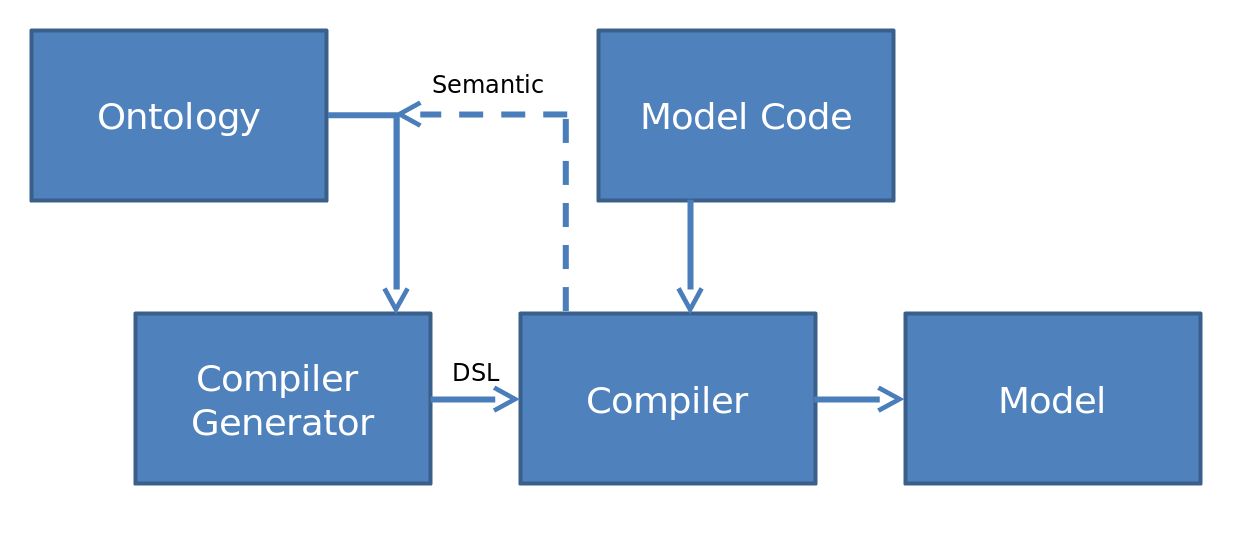
\includegraphics[width=0.8\textwidth]{pics/generation_of_a_dsl/binding1.png}
	\caption{Visualisation of the Dynamic DSL approach \label{fig:visualisation_dyn_dsl}}	
\end{figure}
\par
The idea was to encapsulate this functionality in a component called compiler generator, which searches the ontologies for described entities and generates, depending on them, a grammar with a parser and a compiler that uses the terms of these entities natively. After that step, an IDE could parse the model code the user is writing, and check if it is syntactically correct and may support the user with well known functions as auto completion and so on. The generated compiler is then able to translate the model code directly into machine readable or in a general purpose language like Java, C or C++.
\par
This principal idea is not fundamentally new. There are already existing projects that uses ontologies to create domain specific languages in a dynamic manner. Ceh et. al introduce in \autocite{ontology:ontology2dsl}, \autocite{ontology:onto_in_dsl_dev} the Onto2DSL framework. In \autocite[192]{ontology:onto_in_dsl_dev} they discuss the process of how to translate ontology concepts into grammatical fragments of the dsl in detail and based on an example. Another example is provided in \autocite{ontology:combining_dsl_onto}. They understand ontologies metamodel of the DSL that should be developed. This kind of abstraction of meta levels is based on the Model Driven Architecture (MDA) paradigm. A  more detailed discussion of the MDA approach is out of scope of this work, but interested readers can found a good explanation in \autocite{dsl:mda}. Again the result here is that the DSL is enriched by the semantics of the ontology.
\par
The main problem we see in this approach is, the main component, the compiler generator, which has to dynamically generate the DSL and hence a code generator or compiler. Although we have found examples that give proof that the dynamical generation of a DSL is possible in general, we doubt it that this is possible as an on the fly solution. On the fly means in this case, that the generation of the DSL and the crucial tools to deal with it (code generator, compiler) need to be fully automatic without human rework. Such an on the fly solution would be needed since the user must be able to integrate or generate his own semantical descriptions of entities. In the given examples \autocite{ontology:ontology2dsl}; \autocite{ontology:onto_in_dsl_dev} there is always a DSL engineer involved, that needs to execute several tasks like finding irregularities in the produced grammar and so on.

\subsection{Fixed DSL}
\par
This was the main reason why we tried to work out a conceptual completely different solution. Figure \ref{fig:visualisation_fixed_dsl} depicts the conceptual architecture of this approach.
\begin{figure}[h]
	\centering
	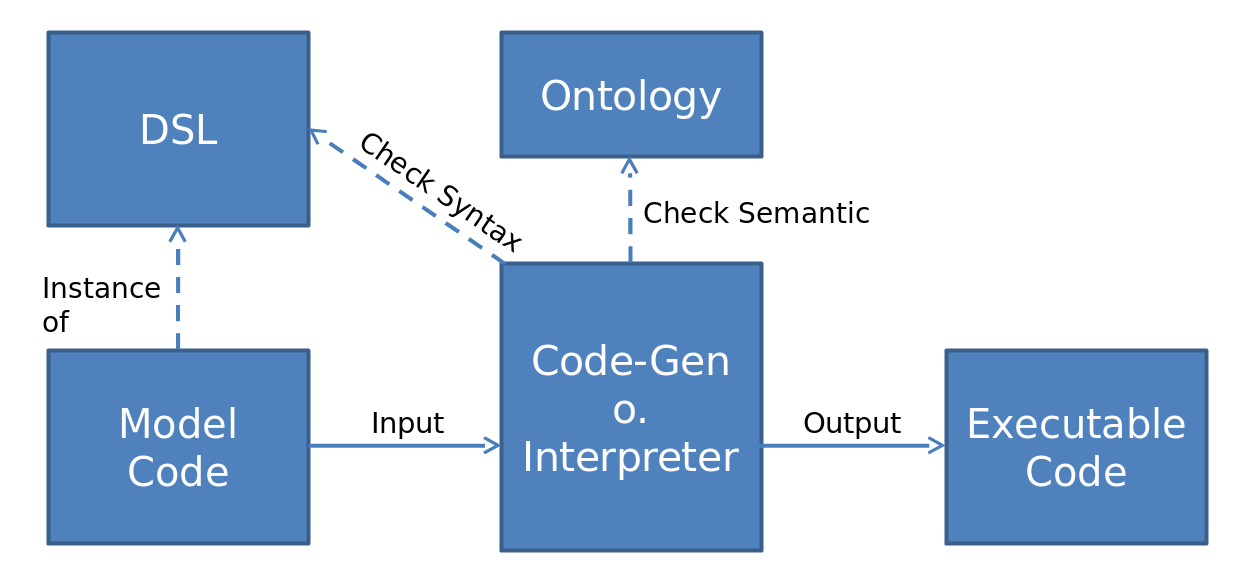
\includegraphics[width=0.8\textwidth]{pics/generation_of_a_dsl/binding2.png}
	\caption{Visualisation of the Fixed DSL approach \label{fig:visualisation_fixed_dsl}}	
\end{figure}

\par
In contrast to the the first solution we decided that a better approach could be to define the DSL in a more general and first and foremost stringent way. This means that the grammar of the DSL would not be dynamic and does not use the terms of semantic entities described in the ontologies natively. Instead it uses them in a generalized form which is a more conventional approach.
\par
Again we use the temperature example of the first approach to explain what this means. In that case temperature is not a lexical element of the DSL but since the meaning of temperature is a datatype the grammar of the DSL would contain a production rule that expresses that a data type consists of several characters.
\par
What is missing is the connection to the ontology. As visualised in Figure \ref{fig:visualisation_fixed_dsl} the connection to the ontology is made by the code generator. Since the code generator is a normal piece of software it is obvious that it is possible to connect to an ontology and use the features and the semantics it provides. Hence this step is more a question of how to design this connection instead of the general possibility. A good possibility to implement the connection between code generator and ontology is based on the fact that it is possible to translate the ontologies into object oriented models and vice versa. In \autocite{ontology:oom_mapping} Athanasiadis describes this transformation process in detail. Furthermore he mentions that ``Several toolkits are available for translating OWL structures into Java classes for supporting coding support for semantic applications'' \autocite[3]{ontology:oom_mapping}.
\par
 In our case this means, that after the definition of semantic data types, an object oriented model (OOM) can be generated, which then can be used by the code generator to generate code that is aware of the semantics defined by the ontologies. This principle would also work the inverse way. For example if the user describes in his model an entity $bank\_account$. The entity bank account has a property $account\_balance$. Furthermore the user has described in an ontology that the account balance of an entity can not be negative. The code generator could use the OOM and generate a $bank\_account$ object which then can be transferred as an individual into the ontology. The ontology itself could then use the automatic reasoning to validate the account balance and throw an error if it does not fulfill the constraint. A very similar approach is implemented in Ocelet. An Ocelet model can be mapped into an ontology and again the reasoning features of the ontology can be used to check constraints.
\par
To sum up, we think that this special part of the larger whole is principally feasible with the approach described above. Of course, there are a lot of open questions and problems left that need to be solved when trying to implement this in reality. For example we did not regard the point that the used ontologies needs to have a pre-defined structure to be able to access ontology semantics such as constraints in the code generator and to reason over modeled entities. For us, it is not clear how many of these problem would appear and even worse, if these implementation specific problems are all solvable. 

























